\subsection{Overall Comparison}
\label{expsec:overall_comparison}

\begin{table}[t]
    \centering
    \caption{\bf 
    Comparison of \sys with baselines on open-source LLMs. The best and second-best results are highlighted in \textbf{bold} and \underline{underlined}, respectively.
    % Results on more LLMs (0.5B, 1.5B, 3B, 7B, 14B models of Qwen2.5 and 0.6B, 1.7B, 4B models of Qwen3) can be found in our technique report~\cite{technical_report}.
    }
    \label{tbl:opensource_exp}
    \vspace{-1em}

    % =======================================================
    % Subtable 5: Open-Source & Training - Qwen3-14B
    % =======================================================
    \begin{subtable}[t]{0.9\columnwidth}
        \centering
        \caption{\bf{Results on Qwen3-14B.}}
        \label{subtbl:open_qwen14b}
        \vspace{-0.5em}
        \resizebox{0.99\linewidth}{!}{
        \begin{tabular}{|c||c|c||c|c|c|c|}
            \hline
            \multirow{2}{*}{\textbf{Method}} & \multicolumn{2}{c||}{\textbf{Synth-Spider}} & \multicolumn{2}{c|}{\textbf{Synth-Bird}} & \multicolumn{2}{c|}{\textbf{Parrot}} \\ \cline{2-7}
             & \textbf{Acc.} & \textbf{Comp.} & \textbf{Acc.} & \textbf{Comp.} & \textbf{Acc.} & \textbf{Comp.} \\
            \hline \hline
            \multicolumn{7}{|c|}{\cellcolor{gray!10}\textit{Prompting Baselines}} \\
            % CodeGen & 41.83 & 67.08\% & 27.74 & 48.71\% & 31.52 & 86.16\% \\
            PaS & 7.67 & 20.67\% & 3.09 & 21.86\% & 9.56 & 22.36\% \\
            MCTS-OP & 21.91 & 72.56\% & 7.22 & {78.69\%} & 24.95 & 83.02\% \\
            MontePrep & 9.46 & 19.62\% & 18.63 & 38.15\% & 26.94 & 57.87\% \\
            AutoPrep & 36.75 & 71.61\% & 10.41 & 39.89\% & 28.54 & 74.05\% \\
            CodeGen & 45.47 & 68.18\% & 29.48 & 49.20\% & 30.83 & 81.08\% \\
            ReAct & 40.39 & 69.02\% & 16.04 & 46.56\% & 30.80 & 76.44\% \\
            \hline \hline
            \multicolumn{7}{|c|}{\cellcolor{gray!10}\textit{Training Methods (Only Trained on Synth-Spider)}} \\
            % IL & \underline{59.61} & \underline{88.65\%} & \underline{44.16} & 74.75\% & \underline{34.58} & 
            IL & \underline{61.70} & \underline{85.26\%} & \underline{48.01} & \underline{81.23\%} & \underline{37.95} & \underline{89.39\%} \\
            RL-GRPO & 51.22 & 77.68\% & 32.25 & 67.22\% & 35.06 & 82.9\% \\ \hline
            \begin{tabular}{@{}c@{}}\textbf{\sys}\\ \textbf{(Ours)}\end{tabular} & \textbf{67.18} & \textbf{97.21\%} & \textbf{54.09} & \textbf{92.26\%} & \textbf{40.44} & \textbf{96.41\%} \\
            \hline
        \end{tabular}
        }
    \end{subtable}

    \vspace{0.5em}
    
    % =======================================================
    % Subtable 4: Open-Source & Training - Qwen3-8B
    % =======================================================
    \begin{subtable}[t]{0.9\columnwidth}
        \centering
        \caption{\bf{Results on Qwen3-8B.}}
        \label{subtbl:open_qwen8b}
        \vspace{-0.5em}
        \resizebox{0.99\linewidth}{!}{
        \begin{tabular}{|c||c|c||c|c|c|c|}
            \hline
            \multirow{2}{*}{\textbf{Method}} & \multicolumn{2}{c||}{\textbf{Synth-Spider}} & \multicolumn{2}{c|}{\textbf{Synth-Bird}} & \multicolumn{2}{c|}{\textbf{Parrot}} \\ \cline{2-7}
             & \textbf{Acc.} & \textbf{Comp.} & \textbf{Acc.} & \textbf{Comp.} & \textbf{Acc.} & \textbf{Comp.} \\
            \hline \hline
            \multicolumn{7}{|c|}{\cellcolor{gray!10}\textit{Prompting Baselines}} \\
            % CodeGen & 29.53 & 45.22\% & 19.12 & 32.52\% & 24.25 & 56.27\% \\
            PaS & 4.68 & 7.42\% & 0.65 & 4.33\% & 3.09 & 8.32\% \\
            MCTS-OP & 12.90 & 15.19\% & 0.90 & 73.56\% & 17.33 & 23.71\% \\
            MontePrep & 8.81 & 19.97\% & 13.70 & 21.96\% & 25.95 & 56.08\% \\
            AutoPrep & 26.44 & 50.85\% & 8.52 & 42.28\% & 25.20 & 70.42\% \\
            CodeGen & 6.27 & 12.10\% & 7.47 & 15.69\% & 7.27 & 25.50\% \\
            ReAct & 29.63 & 52.59\% & 10.41 & 46.22\% & 22.11 & 57.97\% \\
            DeepAnalyze & 35.66 & 82.02\% & 1.74 & 62.17\% & 29.01 & 66.67\% \\
            \hline \hline
            \multicolumn{7}{|c|}{\cellcolor{gray!10}\textit{Training Methods (Only Trained on Synth-Spider)}} \\
            % IL & \underline{58.62} & \underline{92.63\%} & \underline{41.63} & \underline{83.98\%} & \underline{33.26} & \underline{91.36\%} \\ % 2025 Version
            IL & \underline{59.65} & \underline{90.54\%} & \underline{43.30} & \underline{80.43\%} & \underline{36.15} & \underline{91.08\%} \\
            RL-GRPO & 47.81 & 76.54\% & 29.95 & 68.69\% & 32.82 & 85.05\% \\ \hline
            \begin{tabular}{@{}c@{}}\textbf{\sys}\\ \textbf{(Ours)}\end{tabular} & \textbf{65.99} & \textbf{97.46\%} & \textbf{53.39} & \textbf{92.78\%} & \textbf{39.93} & \textbf{98.46\%} \\
            \hline
        \end{tabular}
        }
    \end{subtable}
    \vspace{-1em}
\end{table}

% \begin{table}[t]
    \centering
    \caption{\bf Comparison of \sys and baselines on SOTA LLMs. Results on more LLMs (DoubaoSeed1.6-Thinking, DeepSeek-V3.1 and DoubaoSeed1.6-flash) can be found in our technique report ~\cite{technical_report}.}
    \label{tbl:sota_exp}
    \vspace{-1em}

    % =======================================================
    % Subtable 2: SOTA - Claude-4
    % =======================================================
    \begin{subtable}[t]{\columnwidth}
        \centering
        \caption{\bf{Results on SOTA LLMs (Backbone: Claude-4).}}
        \label{subtbl:sota_claude}
        \vspace{-0.15em}
        \resizebox{0.99\linewidth}{!}{
        \begin{tabular}{|c||c|c|c|c|c|c|}
            \hline
            \multirow{2}{*}{\textbf{Method}} & \multicolumn{2}{c|}{\textbf{DP-Spider}} & \multicolumn{2}{c|}{\textbf{DP-Bird}} & \multicolumn{2}{c|}{\textbf{Parrot}} \\ \cline{2-7}
             & \textbf{Acc.} & \textbf{Comp.} & \textbf{Acc.} & \textbf{Comp.} & \textbf{Acc.} & \textbf{Comp.} \\
            \hline \hline
            CodeGen & 59.51 & 86.65\% & 50.55 & 70.27\% & 40.44 & 91.93\% \\ 
            PaS & 46.91 & 79.83\% & 27.59 & 61.55\% & 41.19 & 93.43\% \\
            MCTS-OP & 66.58 & \underline{99.05\%} & 58.91 & \underline{95.32\%} & 41.68 & 98.51\% \\
            MontePrep & 44.27 & 59.46\% & 26.05 & 45.37\% & 41.93 & 69.72\% \\
            AutoPrep & 63.70 & 97.01\% & 46.71 & 91.24\% & 40.79 & \underline{99.15\%} \\
            CodeGen & 62.05 & 82.82\% & 57.62 & 73.85\% & 41.14 & 92.83\% \\
            ReAct & \underline{69.92} & 96.86\% & \underline{59.91} & 89.09\% & \underline{42.88} & 96.12\% \\
            \hline
            \begin{tabular}{@{}c@{}}\textbf{\sys}\\ \textbf{\textsc{-P} (Ours)}\end{tabular} & \textbf{73.46} & \textbf{99.85\%} & \textbf{67.43} & \textbf{97.91\%} & \textbf{46.07} & \textbf{99.70\%} \\
            \hline
        \end{tabular}
        }
    \end{subtable}

    \vspace{0.5em}

    % =======================================================
    % Subtable 1: SOTA - GPT-5
    % =======================================================
    \begin{subtable}[t]{\columnwidth}
        \centering
        \caption{\bf{Results on SOTA LLMs (Backbone: GPT-5).}}
        \label{subtbl:sota_gpt}
        \vspace{-0.15em}
        \resizebox{0.99\linewidth}{!}{
        \begin{tabular}{|c||c|c|c|c|c|c|}
            \hline
            \multirow{2}{*}{\textbf{Method}} & \multicolumn{2}{c|}{\textbf{DP-Spider}} & \multicolumn{2}{c|}{\textbf{DP-Bird}} & \multicolumn{2}{c|}{\textbf{Parrot}} \\ \cline{2-7}
             & \textbf{Acc.} & \textbf{Comp.} & \textbf{Acc.} & \textbf{Comp.} & \textbf{Acc.} & \textbf{Comp.} \\
            \hline \hline
            CodeGen & 62.90 & 92.73\% & 55.88 & 83.96\% & 38.40 & 93.33\% \\
            PaS & 52.29 & 85.26\% & 36.65 & 73.85\% & 39.39 & 95.32\% \\
            MCTS-OP & 61.55 & \underline{97.41\%} & 47.71 & \textbf{95.02\%} & 33.72 & \textbf{99.20\%} \\
            MontePrep & 41.09 & 65.14\% & 27.14 & 51.00\% & \textbf{42.98} & 85.21\% \\
            AutoPrep & 51.54 & 82.87\% & 45.42 & 79.63\% & 38.25 & 85.96\% \\
            CodeGen & 64.39 & 92.38\% & 56.82 & 89.89\% & 40.29 & 95.72\% \\
            ReAct & \underline{67.03} & 97.31\% & \underline{57.37} & \underline{93.38\%} & 40.19 & {96.36\%} \\ % re-run the exp
            \hline
            \begin{tabular}{@{}c@{}}\textbf{\sys}\\ \textbf{\textsc{-P} (Ours)}\end{tabular} & \textbf{71.76} & \textbf{98.21\%} & \textbf{60.46} & 92.53\% & \underline{41.33} & \underline{97.26\%} \\
            \hline
        \end{tabular}
        }
    \end{subtable}

    \vspace{0.5em}

    % =======================================================
    % Subtable 3: SOTA - DeepSeek-R1
    % =======================================================
    \begin{subtable}[t]{\columnwidth}
        \centering
        \caption{\bf{Results on SOTA LLMs (Backbone: DeepSeek-R1).}}
        \label{subtbl:sota_dsr1}
        \vspace{-0.15em}
        \resizebox{0.99\linewidth}{!}{
        \begin{tabular}{|c||c|c|c|c|c|c|}
            \hline
            \multirow{2}{*}{\textbf{Method}} & \multicolumn{2}{c|}{\textbf{DP-Spider}} & \multicolumn{2}{c|}{\textbf{DP-Bird}} & \multicolumn{2}{c|}{\textbf{Parrot}} \\ \cline{2-7}
             & \textbf{Acc.} & \textbf{Comp.} & \textbf{Acc.} & \textbf{Comp.} & \textbf{Acc.} & \textbf{Comp.} \\
            \hline \hline
            CodeGen & 56.23 & 86.11\% & 52.09 & 76.99\% & 36.06 & 93.53\% \\
            PaS & 44.92 & 72.66\% & 34.41 & 51.34\% & 35.86 & 89.69\% \\
            MCTS-OP & \underline{62.10} & \textbf{96.07\%} & 50.85 & \textbf{95.77\%} & 33.02 & 95.32\% \\
            MontePrep & 33.52 & 53.54\% & 17.63 & 33.22\% & \textbf{42.58} & 82.77\% \\
            AutoPrep & 54.53 & 84.61\% & 40.09 & 89.49\% & 33.17 & 96.96\% \\
            CodeGen & 59.71 & 78.09\% & 45.27 & 65.49\% & 35.91 & 88.30\% \\
            ReAct & 59.11 & 85.91\% & \underline{59.31} & \underline{89.64\%} & 38.84 & \underline{97.21\%} \\ 
            \hline
            % \textbf{\sys-P (Ours)} & \textbf{65.23} & \underline{93.92\%} & \textbf{60.16} & 88.65\% & \underline{39.64} & \textbf{98.26\%} \\
            \begin{tabular}{@{}c@{}}\textbf{\sys}\\ \textbf{\textsc{-P} (Ours)}\end{tabular} & \textbf{65.23} & \underline{93.92\%} & \textbf{60.16} & 88.65\% & \underline{39.64} & \textbf{98.26\%} \\
            \hline
        \end{tabular}
        }
    \end{subtable}

    
\end{table}


% \begin{figure}[t]
    \centering
    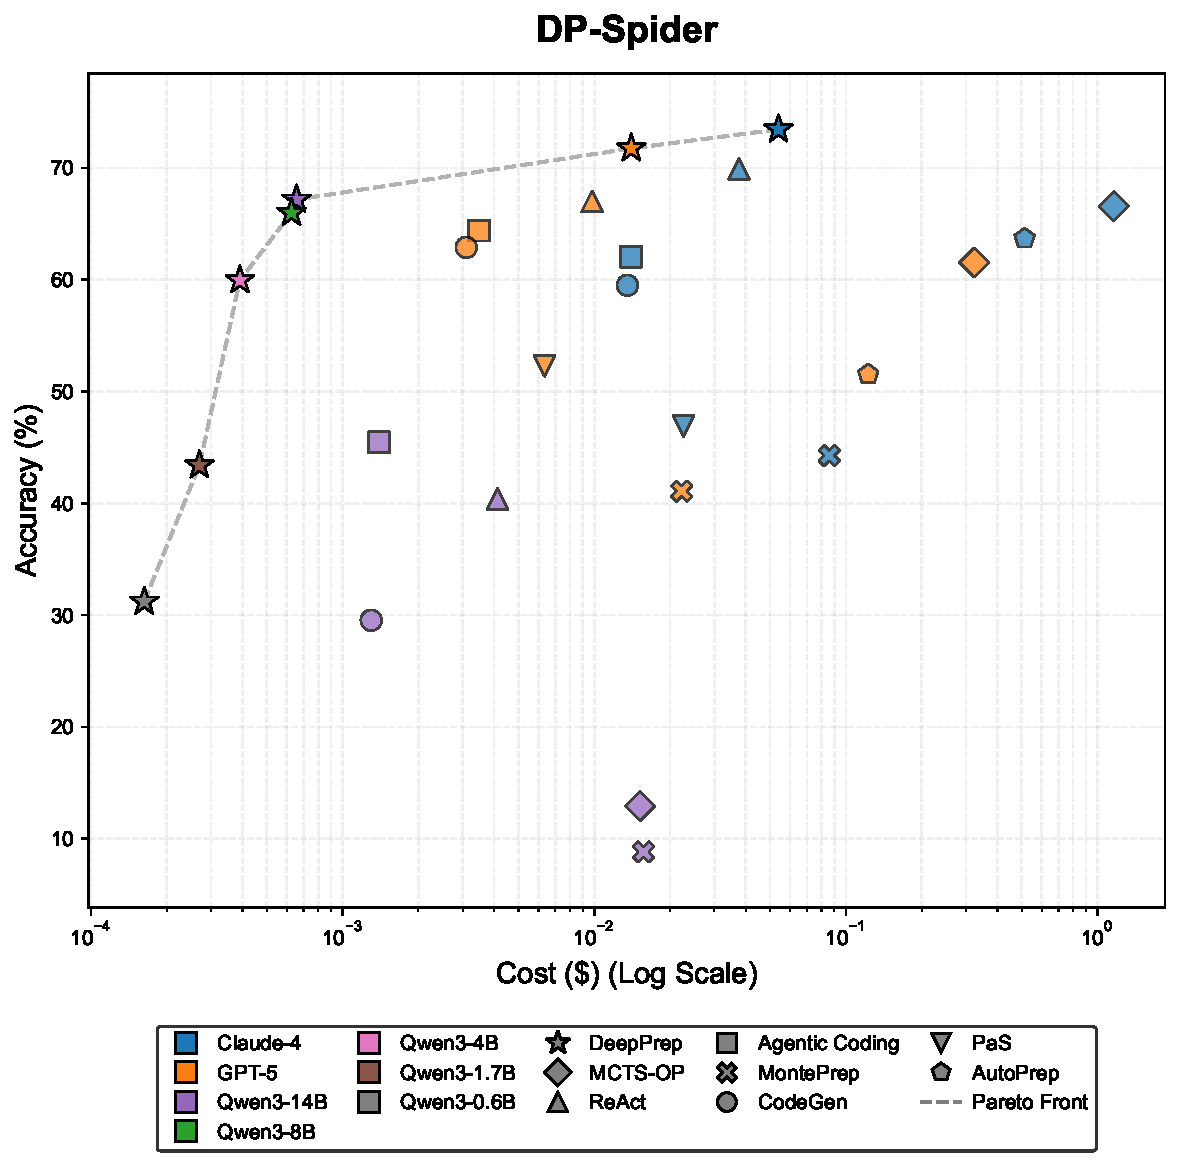
\includegraphics[width=0.99\columnwidth]{plots/plot/pareto_front_spider.pdf}
    \vspace{-1em} 
    \caption{Pareto Front on DP-Spider.}
    \label{fig:pareto_front_spider}
    % \vspace{-1em}
\end{figure}
% \begin{figure}[t]
    \centering
    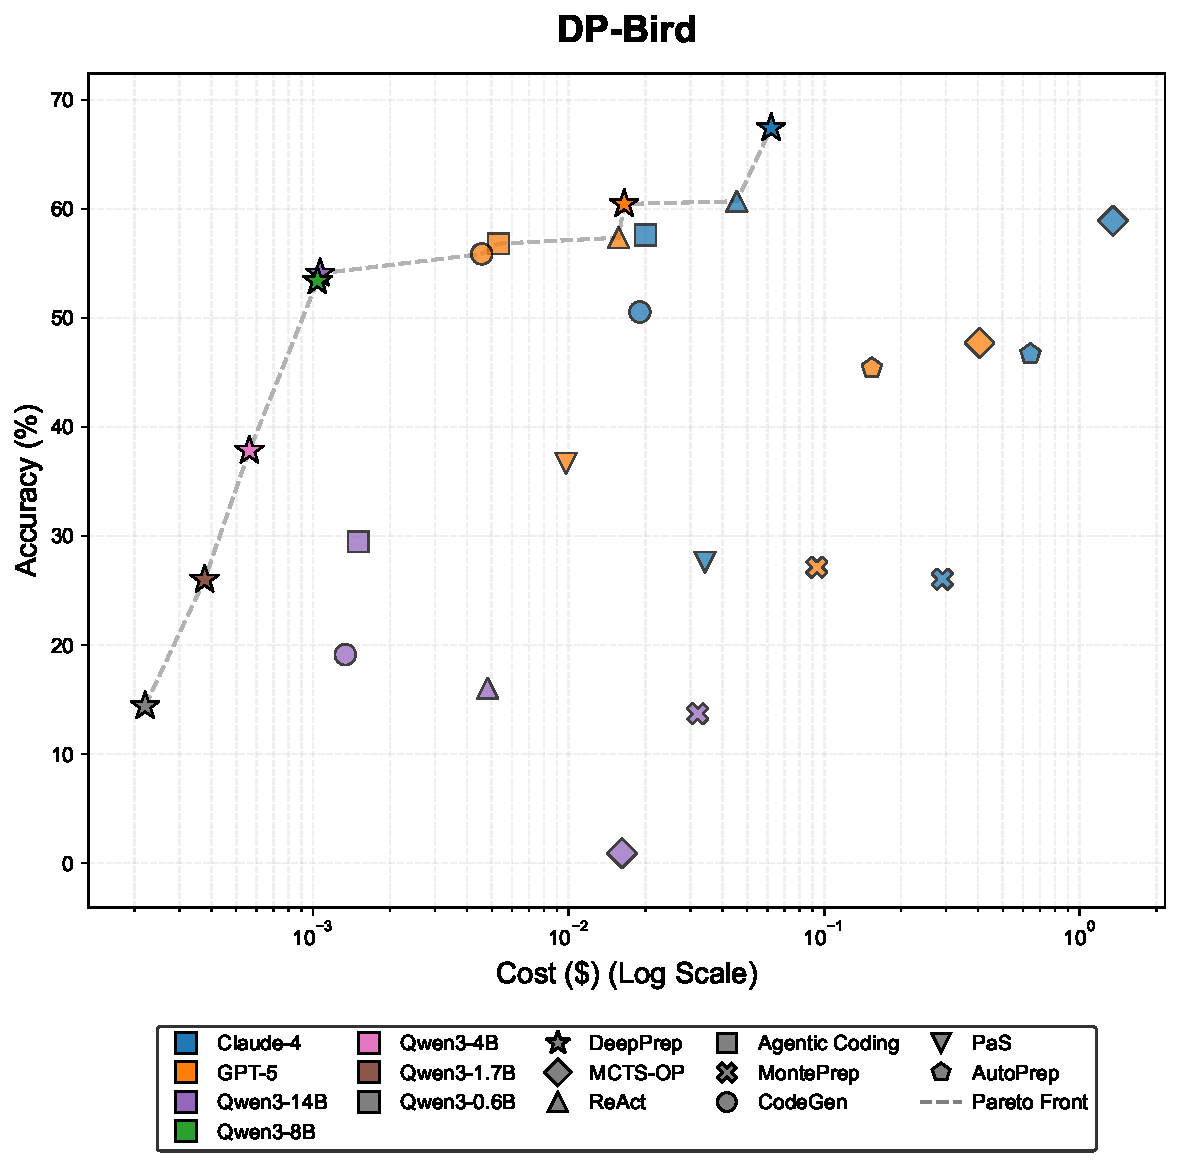
\includegraphics[width=0.99\columnwidth]{plots/plot/pareto_front_bird.pdf}
    \vspace{-1em} 
    \caption{Pareto Front on DP-Bird.}
    \label{fig:pareto_front_bird}
    % \vspace{-1em}
\end{figure}
% \begin{figure}[t]
    \centering
    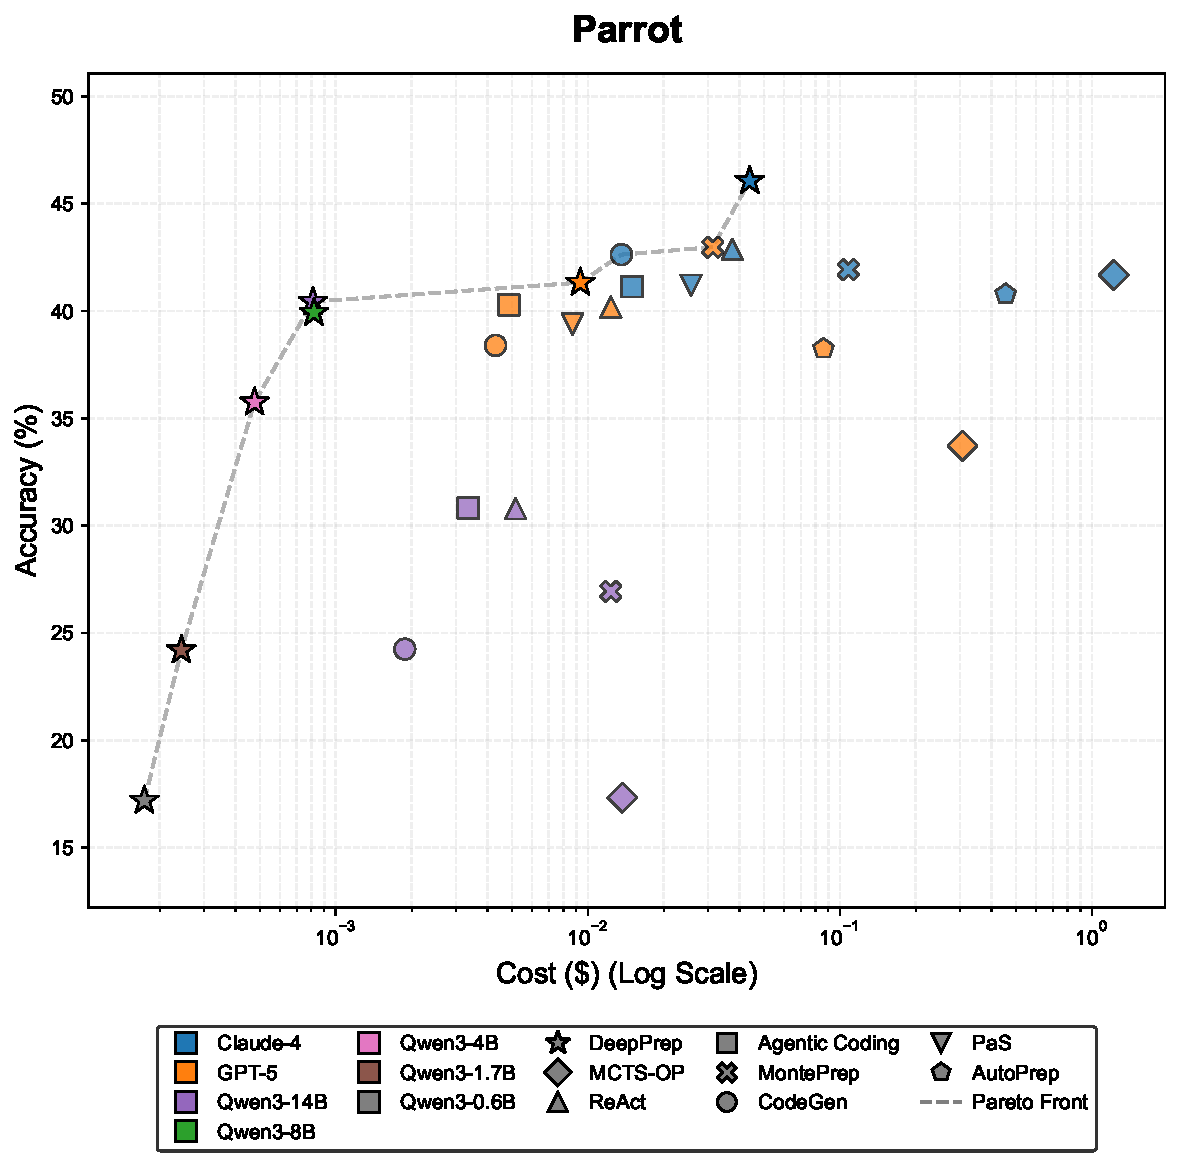
\includegraphics[width=0.99\columnwidth]{plots/plot/pareto_front_parrot.pdf}
    \vspace{-1em} 
    \caption{Pareto Front on Parrot.}
    \label{fig:pareto_front_parrot}
    % \vspace{-1em}
\end{figure}
%!TEX root = ../../main.tex
\begin{figure*}[t]
    \centering 
    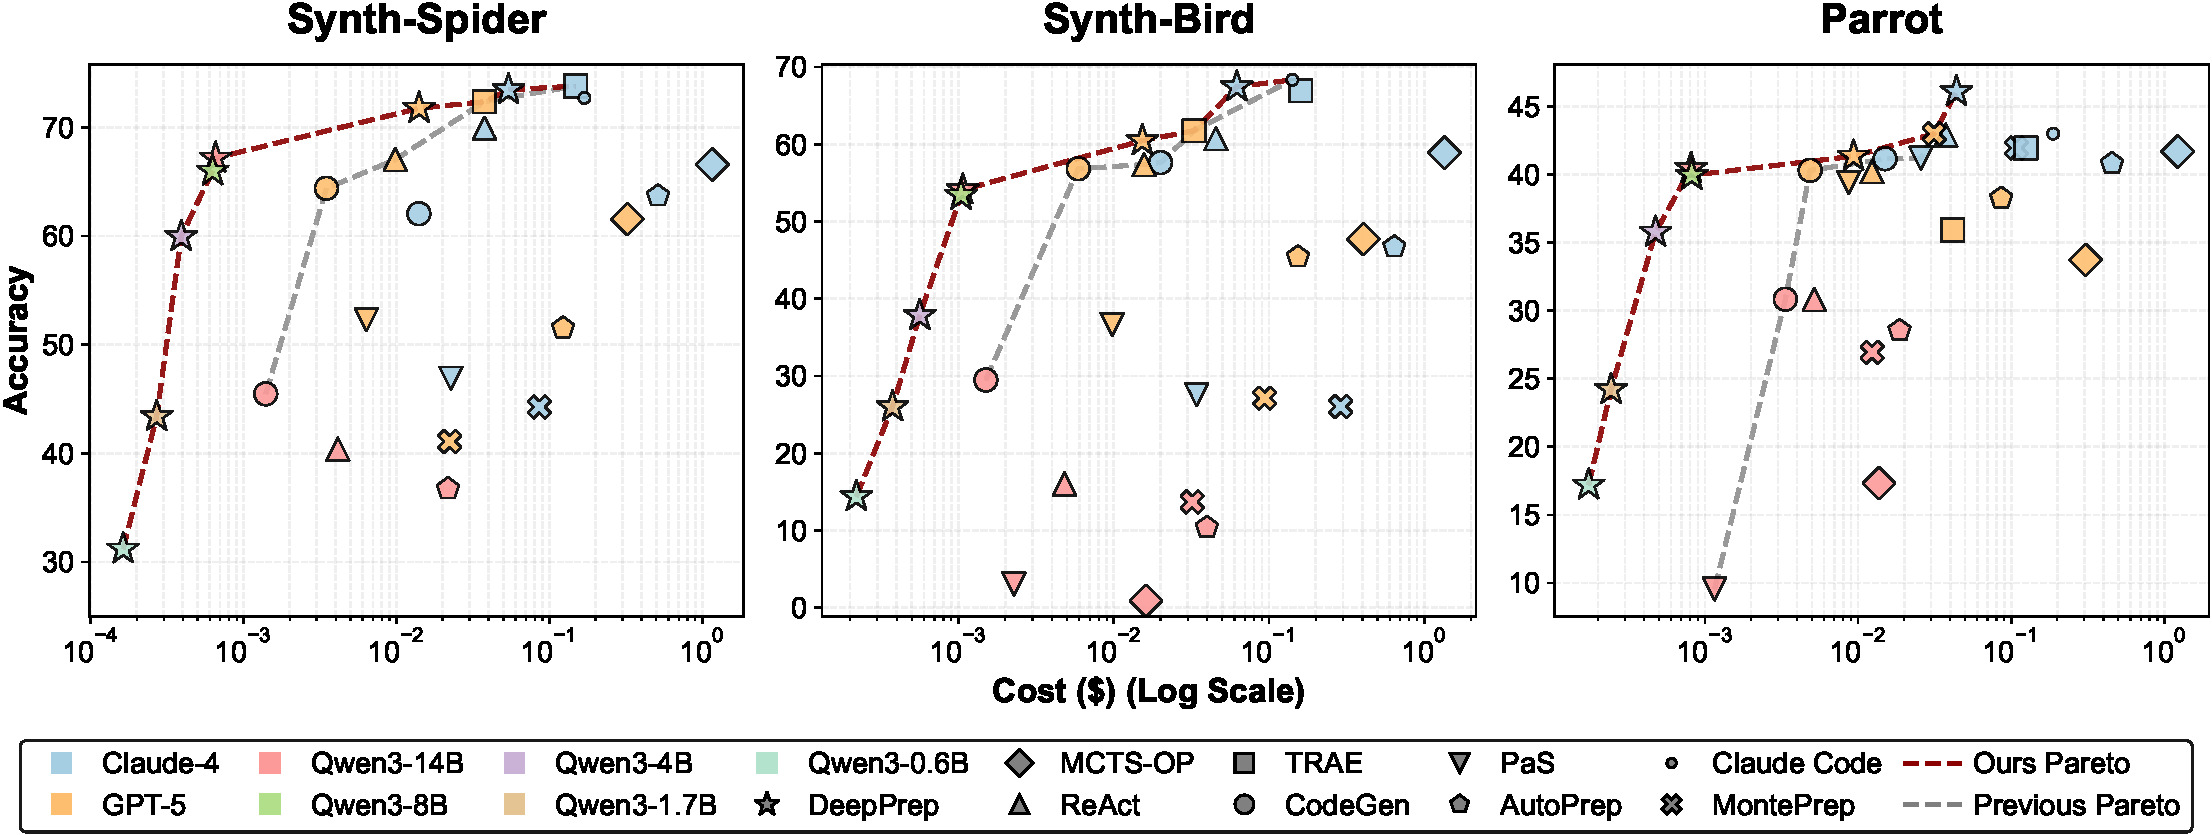
\includegraphics[width=0.7\textwidth]{plots/plot/combined_pareto_front_compare.pdf}
  \vspace{-0.7em}
    \caption{Cost–Accuracy trade-off comparison. Colors represent different LLM backbones, and shapes denote different methods. The red and grey dashed lines indicate the Pareto frontiers of our method and previous baselines, respectively.
    }
    \label{fig:combined_pareto_front_compare}
  \vspace{-1em}
\end{figure*}  



\noindent
\textbf{Exp-\expnum\label{exp:training_comparison}: Comparison of \sys with prompting and training baselines.}
We evaluate the effectiveness of our training strategies by comparing \sys with extensive prompting baselines and training baselines. The results on Qwen3-14B and Qwen3-8B are presented in Table~\ref{tbl:opensource_exp}.

First, \sys establishes new SOTA results. As shown in Table~\ref{subtbl:open_qwen14b}, \sys (Qwen3-14B) achieves an accuracy of \textbf{67.18} on DP-Spider. This significantly outperforms the best prompting baseline AgenticCoding by a margin of 21.71. Furthermore, it surpasses the standard SFT baseline. Specifically, as shown in Table~\ref{subtbl:open_qwen8b}, \sys (Qwen3-8B) achieves higher Accuracy than SFT baselines on Qwen3-14B, with an improvement by 4.29 points. This validates that by adopting the policy training strategy on the synthesized data, we can unleash the agentic tree-based reasoning capability of small-size open-source LLMs.

Second, \sys exhibits robust generalization capabilities under the \textit{single-source training, multi-target evaluation} setting. On the complex cross-domain dataset DP-Bird, \sys consistently widens the performance gap against SFT on both backbones. Specifically, \sys (Qwen3-14B) achieves 54.09 accuracy, outperforming SFT (48.01) by a margin of 6.08 points. Similarly, the 8B model achieves 53.39 accuracy, maintaining a strong lead over its SFT baseline (43.30). This indicates that \sys learns the intrinsic reasoning logic of DP rather than merely memorizing schema-specific patterns from the training set. % 而非学到特定模式

Third, \sys significantly outperforms general-purpose data agents. We observe that DeepAnalyze (Table~\ref{subtbl:open_qwen8b}) struggles in data preparation. While it achieves moderate performance on DP-Spider (35.66), its accuracy collapses to 1.74 on DP-Bird. This failure highlights the necessity of a dedicated DP agent. General agents lack the specialized domain knowledge required to handle multi-hop table transformations. In contrast, \sys leverages high-quality synthesized trajectories to master these domain-specific challenges.

\begin{shaded}
\noindent \textbf{Finding \findingnum: \sys achieves best performance on both 8B and 14B scales and demonstrating strong generalization capabilities.}
\end{shaded}

\noindent \textbf{Exp-\expnum\label{exp:prompting_comparison}: Comparison of \sysp with prompting baselines on SOTA LLMs.}
We compare \sysp with various prompting baselines across three datasets using three SOTA LLM backbones. The detailed results are reported in Table~\ref{tbl:sota_exp}. 

First, \sysp consistently achieves the highest accuracy on complex domain-specific datasets. As shown in Table~\ref{subtbl:sota_claude}, with the Claude-4 backbone, \sysp achieves \textbf{73.46} accuracy on DP-Spider and \textbf{67.43} on DP-Bird. This significantly outperforms the strongest linear baseline, ReAct, by margins of 3.54 and 7.52 respectively. Similarly, on the DeepSeek-R1 backbone (Table~\ref{subtbl:sota_dsr1}), \sysp maintains its lead with \textbf{65.23} accuracy on DP-Spider compared to MCTS-OP (62.10). This performance gain stems from our operator-assisted agentic tree framework. Our framework leverages a global state tree. This structure enables divide-and-conquer strategies that effectively decompose complex, multi-hop DP requirements into manageable sub-tasks.

Second, \sysp demonstrates superior robustness and stability compared to search-based methods. \sysp maintains high performance across all datasets and backbones. In contrast, the performance of MontePrep collapses on complex tasks like DP-Bird (dropping to 27.14). This indicates that \sysp does not rely on chance or dataset-specific heuristics. Instead, it sysematically explores the solution space using the predefined operator set.

Third, \sysp exhibits significantly higher complete rate than linear baselines, particularly on weaker backbones or difficult tasks. On DeepSeek-R1 (Table~\ref{subtbl:sota_dsr1}), \sysp achieves a 93.92\% compilation rate on DP-Spider, whereas ReAct drops to 85.91\% and MontePrep to 53.54\%. This advantage is attributed to the backtracking capability of our agentic tree-based reasoning. Linear methods like AgenticCoding and ReAct suffer from irreversible error propagation where one incorrect step invalidates the entire script. While \sysp detects execution failures at intermediate nodes and backtracks to alternative paths.

\begin{shaded}
\noindent \textbf{Finding \findingnum: \sysp achieves the overall best Accuracy while consistently maintaining a high Completion Rate (>88\%) across diverse LLM backbones.}
\end{shaded}